\documentclass[a4paper,12pt]{article}

% Any percent sign marks a comment to the end of the line

% Every latex document starts with a documentclass declaration like this
% The option dvips allows for graphics, 12pt is the font size, and article
%   is the style

\usepackage[pdftex]{graphicx}
%\usepackage{url}
\usepackage{hyperref}
% These are additional packages for "pdflatex", graphics, and to include
% hyperlinks inside a document.
\usepackage{lettrine}
%\setlength{\oddsidemargin}{0.25in}
%\setlength{\textwidth}{6.5in}
%\setlength{\topmargin}{0in}
%\setlength{\textheight}{8.5in}

% These force using more of the margins that is the default style
\usepackage{times}
\usepackage{mathptmx}
\usepackage{color}
\usepackage{amssymb}
\usepackage{amsmath}
\usepackage{indentfirst}
\usepackage{float}
\begin{document}

% Everything after this becomes content
% Replace the text between curly brackets with your own

\title{Spring 2018 CS304 Software Engineering\\Function as a Service}
\author{Ziqiang Li\quad Yulian Mao\quad Xizi Ni\quad Yilin Zheng\quad Chenyu Zhou\\
\small \{11510352, 11510086, 11510602, 11510506, 11510374\}@mail.sustc.edu.cn\\
Stone Tencent\\
Yuqun Zhang\quad zhangyq@sustc.edu.cn}
\date{\today}

% You can leave out "date" and it will be added automatically for today
% You can change the "\today" date to any text you like


\maketitle

% This command causes the title to be created in the document

\section{Abstract}
Serverless computing is recently raised hot fields of cloud computing. Serverless computing can hide the implementation of the back end from developers or users by using API gateway. The FaaS is a widely used model of serverless computing. In this project, we focus on developing serverless cloud functions(SCF) based on Tencent Cloud to provide a service for massive data, such as image processing. This service will finally be developed into to-business APIs with comprehensive documents.

\section{Review}
This part will roughly review some concepts to help better summarize our project. The concepts related to FaaS includes \textit{serverless computing}, \textit{function as a service}, \textit{API Gateway}.  

\subsection{Serverless Computing}
Serverless computing is a cloud computing model in which the cloud provider dynamically manages the allocation of machine resources. The pricing is based on the actual amount of resources consumed by an application or requests, instead of the units of capacity. Serverless computing does not mean no servsers, it still requires servers. The name "serverless computing" is used because the server management and capacity planning decisions are completely hidden from the developers or operators. Serverless code can be used in conjunction with code deployed in traditional styles, such as microservices. Alternatively, applications can be written to be purely serverless and use no provisioned servers at all\cite{serverless}.

\subsection{Function as a Service}
Function as a service (FaaS) is a category of cloud computing services that provides a platform allowing customers to develop, run, and manage application functionalities without the complexity of building and maintaining the infrastructure typically associated with developing and launching an app. Building an application following this model is one way of achieving a "serverless" architecture, and is typically used when building microservices applications\cite{faas}. 

The advantages of FaaS:
\begin{itemize}
	\item Lower cost: save infrastructure costs, personnel cost, and development costs
	\item Strong expandability
	\item Simpler management
	\item High resource utilization
\end{itemize}

\subsection{API Gateway}

The Figures~\ref{fig:apigateway} shows the simple structure of API Gateway.
\begin{figure}[H]
\centering
\label{fig:apigateway}
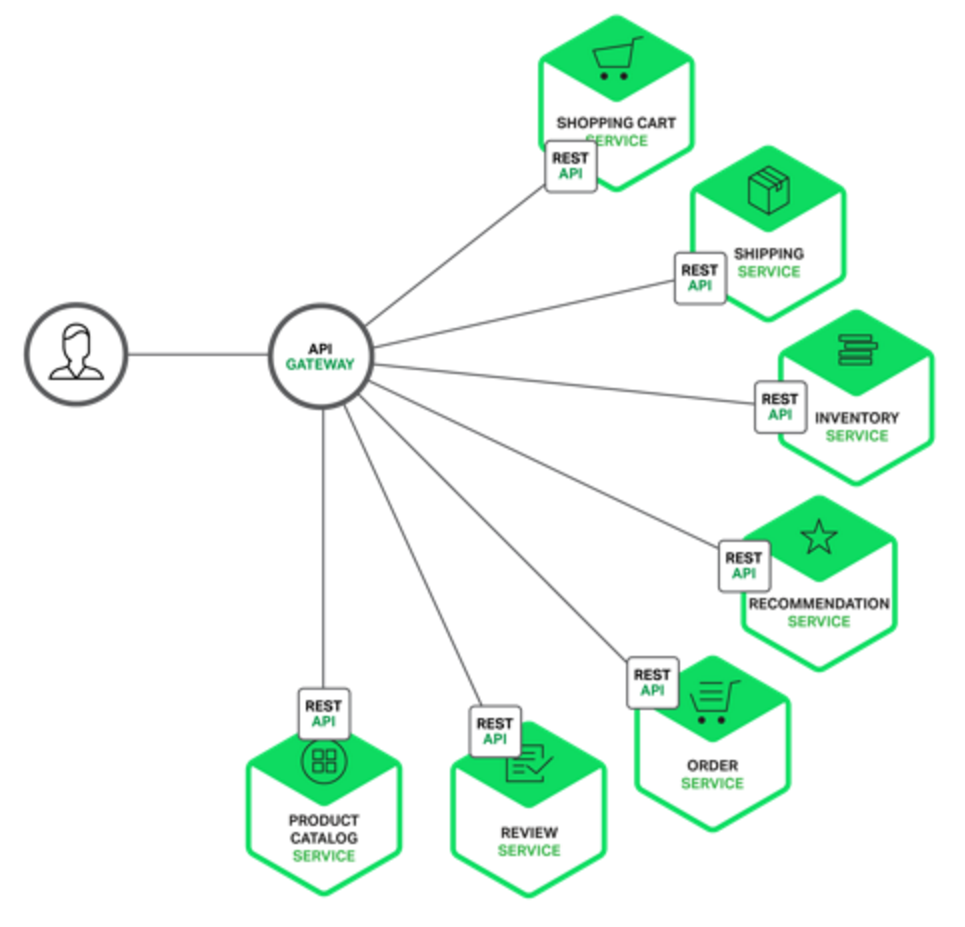
\includegraphics[scale=0.22]{figures/api-gateway.png}
\caption{API Gateway}
\end{figure}

\section{Features and Requirements}
Our project is based on the problem that traditional service cannot handle a sharp increment of computing caused by large concurrent requests. It means, some situations have unstable computing requirements according to time or something others. This project is developed in order to deal with the unstable user demand. The providers can not expend their server unlimited. Therefore, the FaaS is suitable for their scenario. Based on this background, the stakeholder required us to implement some figure processing cloud function such as:
\begin{itemize}
    \item Zoom out
    \item Rotation
    \item Compression
    \item Watermark (words/figures)
    \item Round Corner
    \item Overlap QR Codes
    \item Index Cutting
    \item Format	Conversion
\end{itemize}

Besides, those functions are highly customized. Users can adjust many parameters to meet their own demand. These services are based on Tencent Cloud which is a strong back end. 

The product is now planned to shift to face business customers and provides stable APIs in future. 

\section{Design and Architecture}

The architecture can be referred as \ref{fig:diagram}.

\begin{figure}[H]

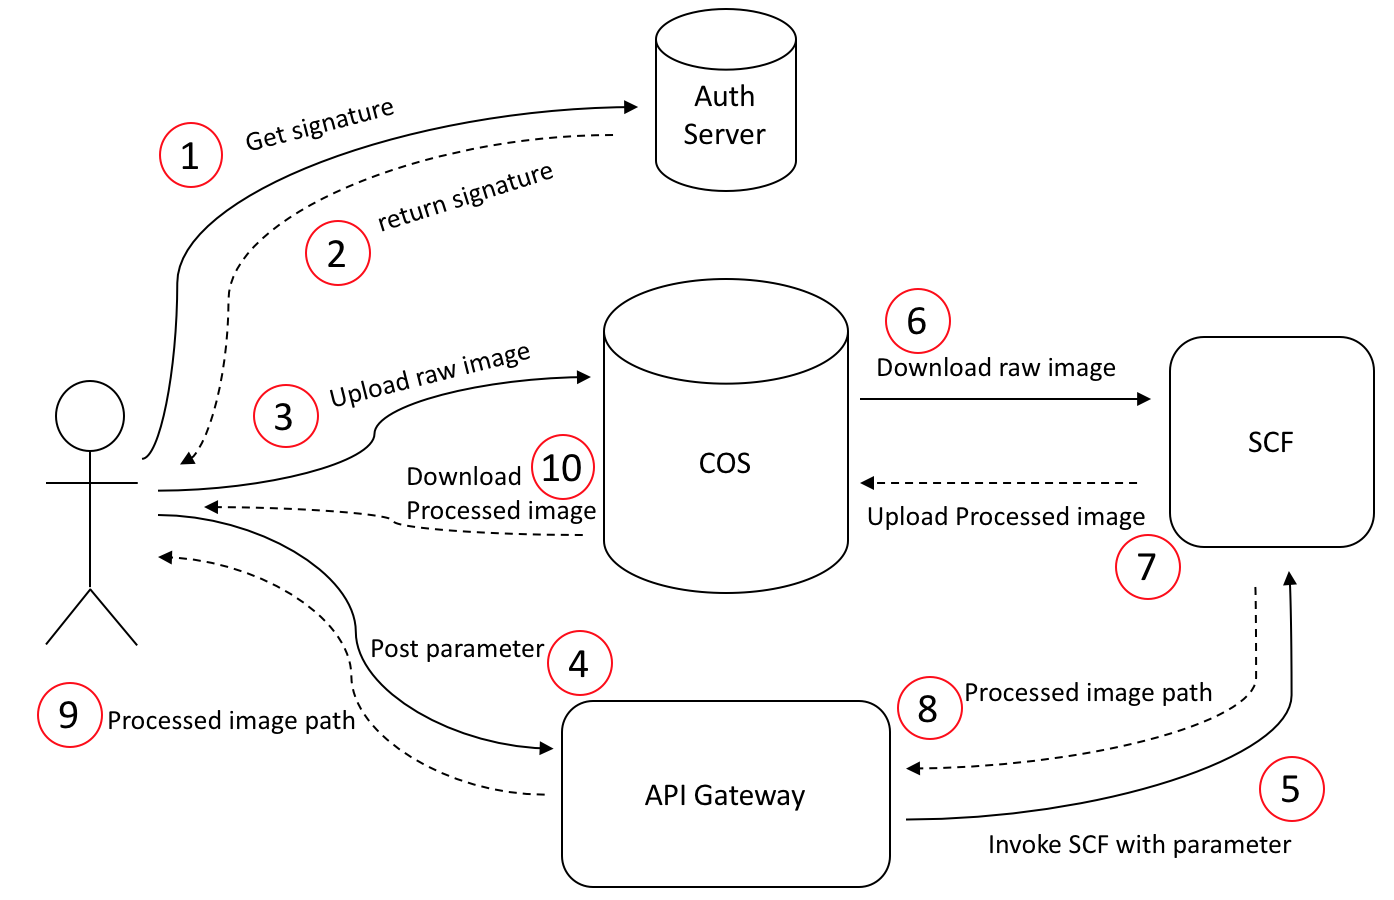
\includegraphics[scale=0.6]{figures/architecture.png}
\caption{\label{fig:diagram}Architecture}
\end{figure}

We use Tencent Cloud SCF service to develop our cloud function, use their COS to store figures and use API Gateway to custom our APIs to release to users. 

The workflow includes:

\begin{enumerate}
	\item Get the authorized secret key to upload the image

	For safety reasons, the user cannot get the authorization for uploading the image as the administrator. Users’ image will be checked and users will be returned an authorized signature for uploading an image to COS.
	\item Upload image with the signature
	
	User upload image with the signature.

	\item Post parameter to image processing
	
	User post the image processing query to the API, which includes the parameters. A processed image path will be returned.
	
	\item Download processed image
	
	The user can preview or download the processed image from the previous path.

\end{enumerate}

\section{Implementation}

\subsection{Team assignment}

\begin{itemize}
	\item Front End: Yulian Mao, Chenyu Zhou
	\item Back End: Ziqiang Li, Xizi Ni, Yilin Zheng
	\item Documentation: Yilin Zheng, Ziqiang Li
	\item Reports: Yilin Zheng
	\item PPTs: Xizi Ni, Yilin Zheng
\end{itemize}

\subsection{Platform choices}
	The platform we choices includes Tencent Cloud Servers, API Gateway, and COS Object storage. The system is Linux.


\section{User Interface}
We have developed a comprehensive documents on \textit{Github pages} and \textit{Readthedocs} with \textit{Sphinx}. The full document can be access from:
\begin{itemize}
	\item Github pages: \url{faasdev.github.io}
	\item Readthedocs: \url{https://faasdevgithubio.readthedocs.io}
\end{itemize}

\section{Conclusion}
This project is a serverless function development based on Tencent Cloud. This service provides basic image processing, and can be further added more SCFs if necessary. This service is serverless so the users have not burden of managing and maintaining servers. Besides, the pricing is counted by the times of requests but not whole servers which largely saves their cost. We have planned to further develop this service to APIs for business. 

\appendix

\section{Demo}



\section{Documents}
\begin{figure}[H]
\centering
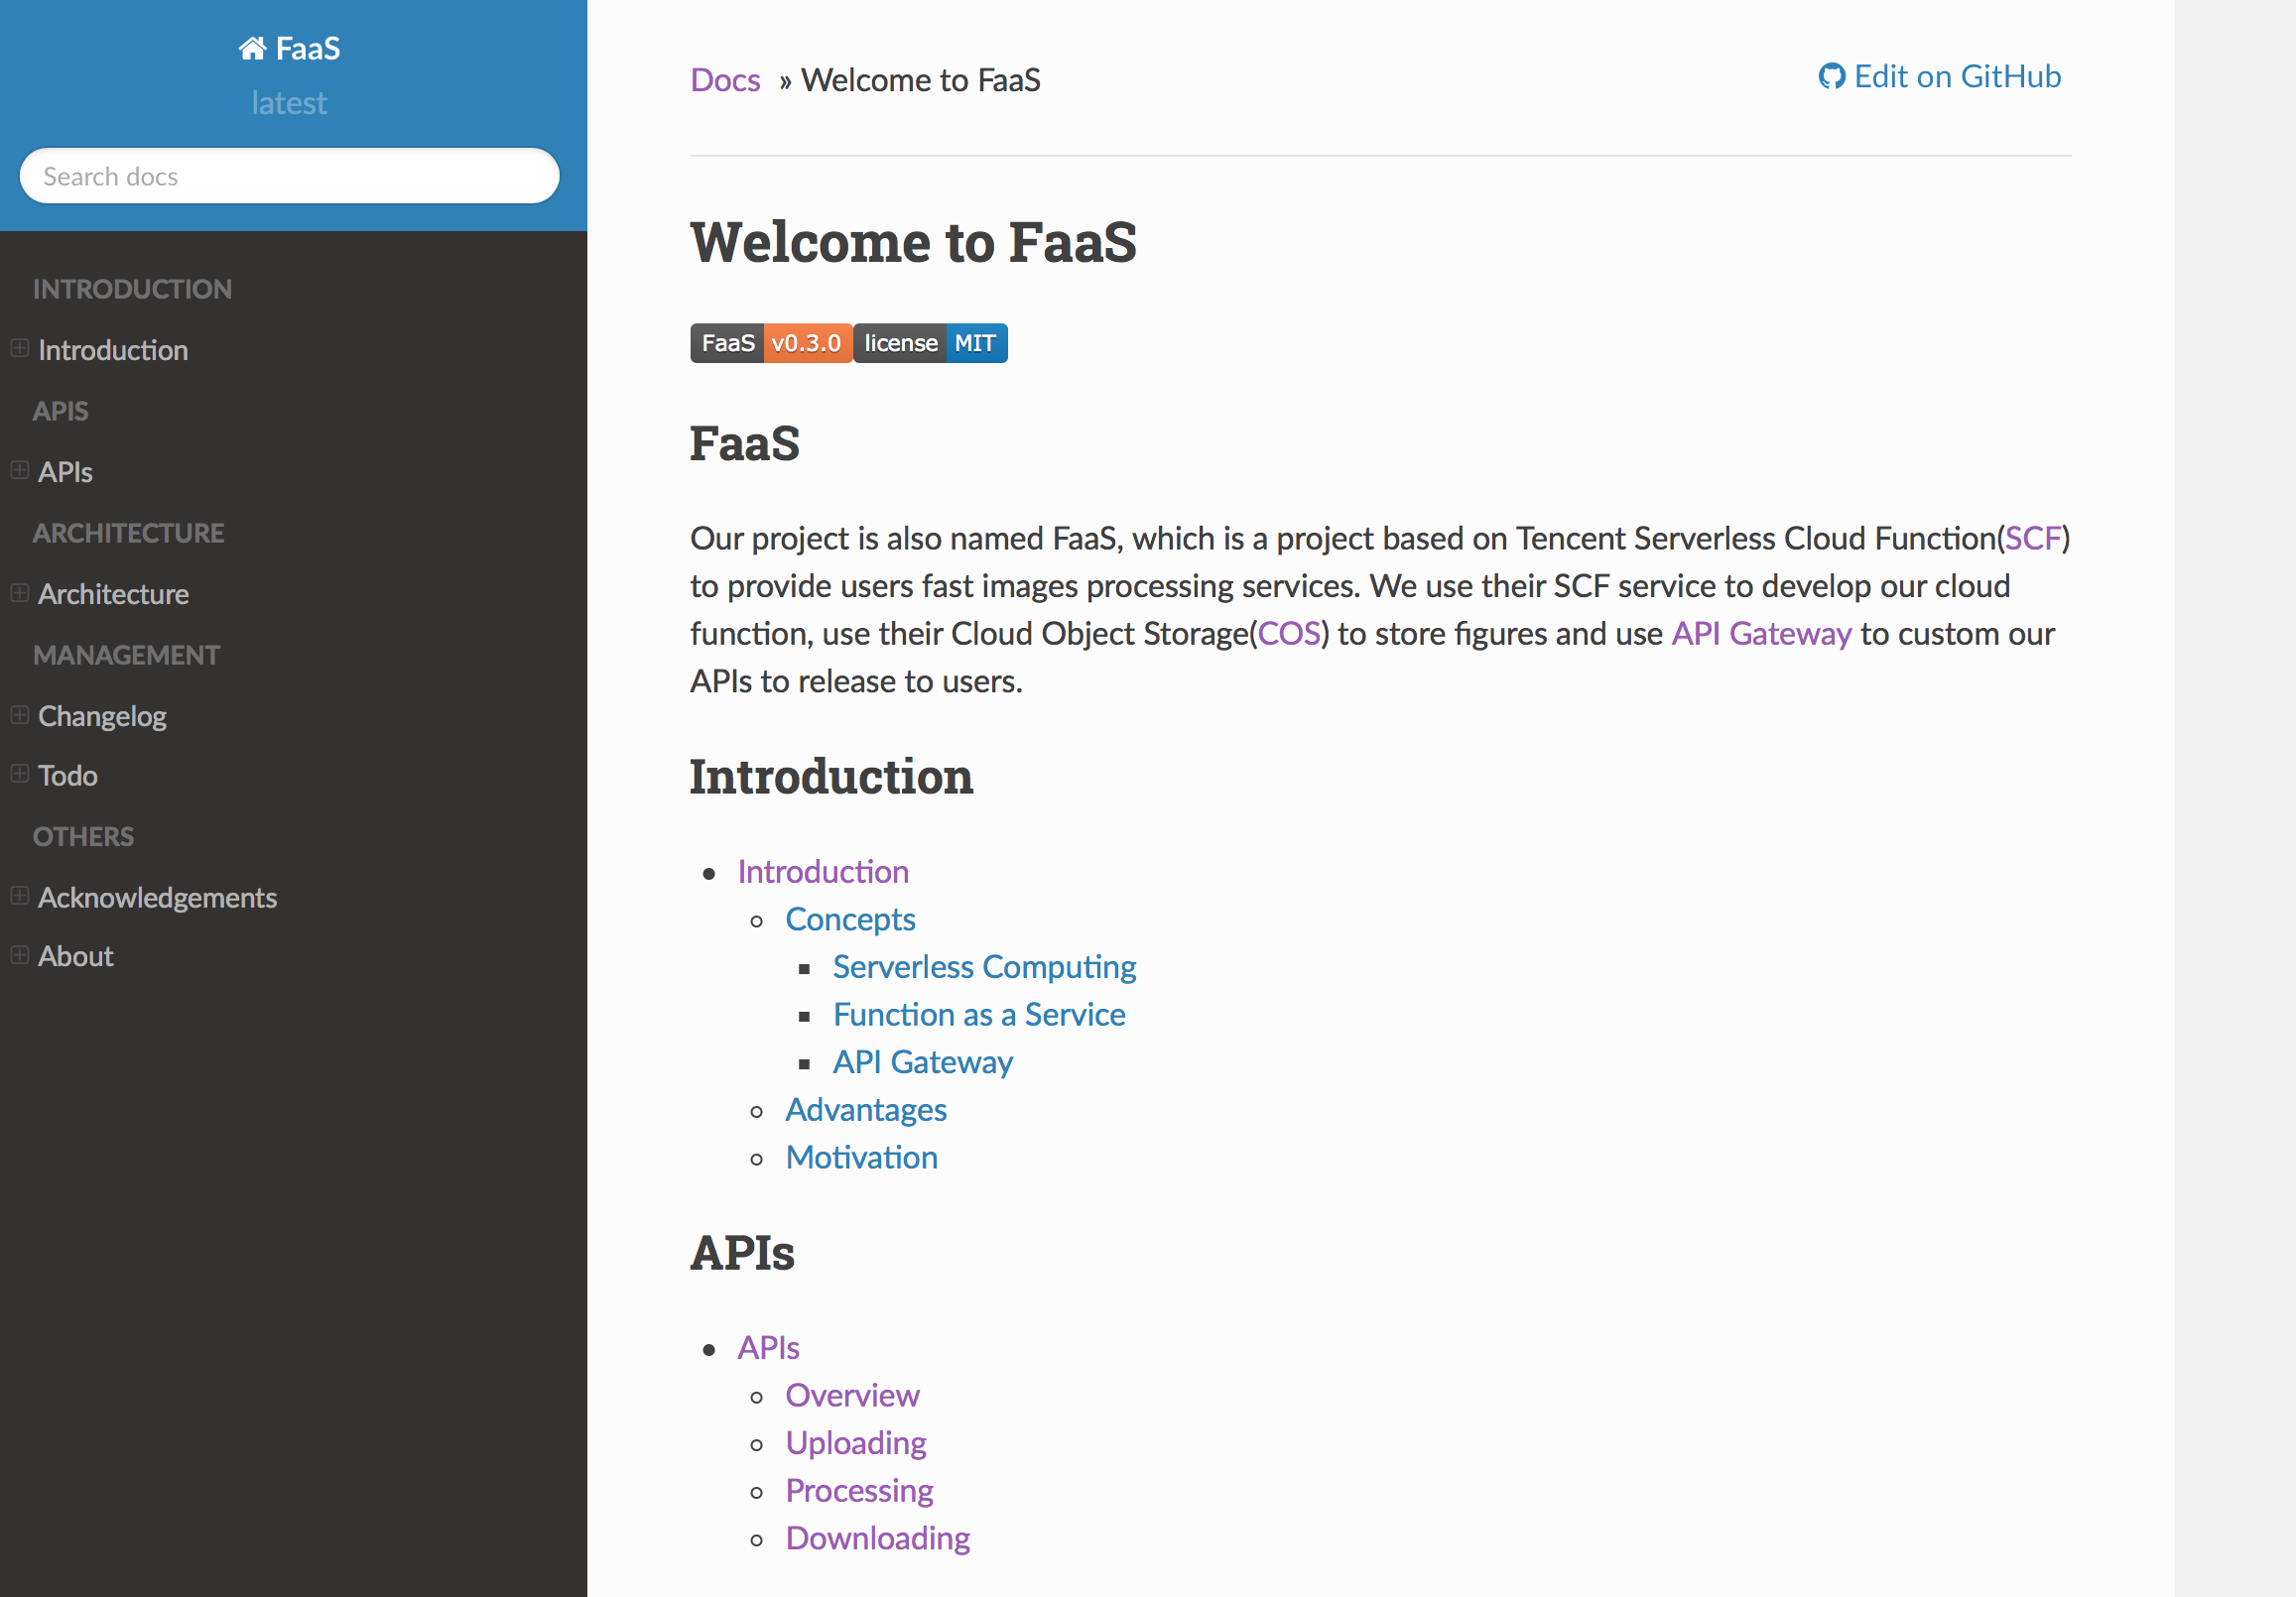
\includegraphics[scale=0.36]{figures/docs1.png}
\caption{\label{fig:docs1}Document}
\end{figure}

\begin{figure}[H]
\centering
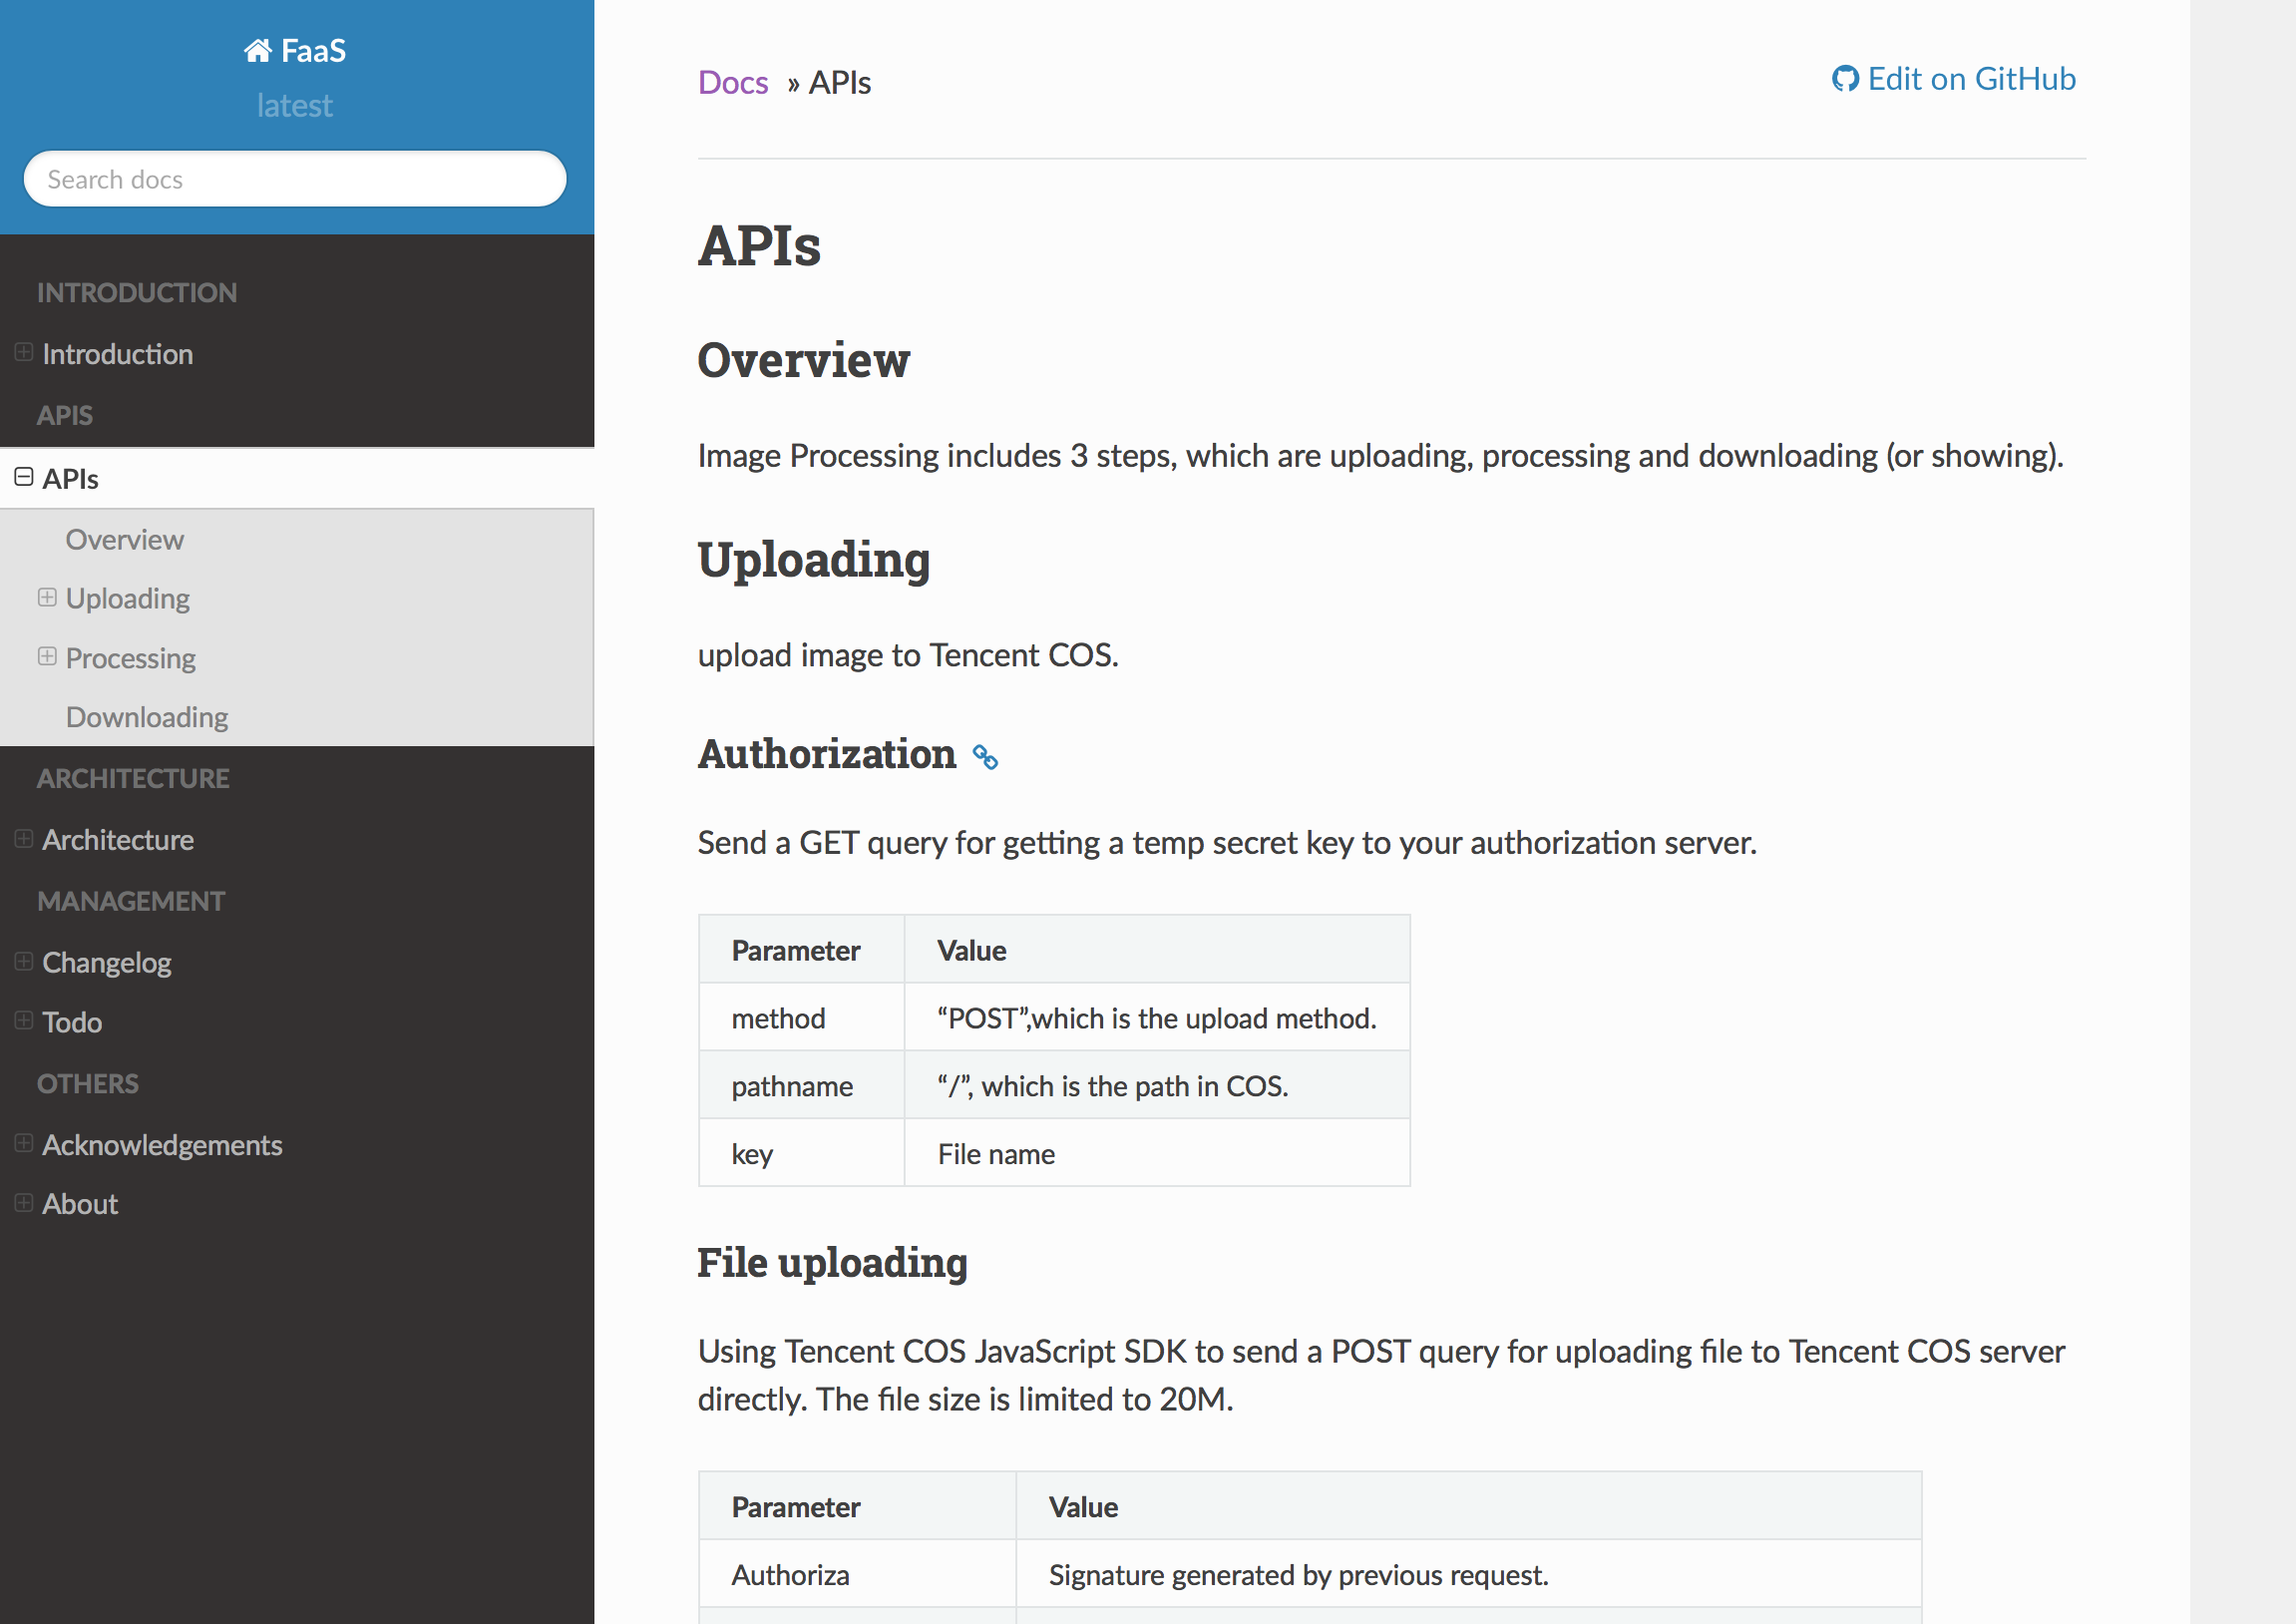
\includegraphics[scale=0.36]{figures/docs2.png}
\caption{\label{fig:docs2}Document}
\end{figure}



\begin{thebibliography}{1}
\bibitem{serverless}
https://en.wikipedia.org/wiki/Serverless\_computing
\bibitem{faas}
https://en.wikipedia.org/wiki/Function\_as\_a\_service
\bibitem{models}
https://mesosphere.com/blog/iaas-vs-caas-vs-paas-vs-faas/

\end{thebibliography}
\end{document}
